%%%%%%%%%%%%%%%%%%%%%%%%%%%%%%%%%%%%%%%%%%%%%%%%%%%%%%%%%%%%%%%%%%%%%%%%%%%%%%%%%%%%
% Do not alter this block (unless you're familiar with LaTeX)
\documentclass{../labbook}
\usepackage{graphicx}
\usepackage{float}
%%%%%%%%%%%%%%%%%%%%%%%%%%%%%%%%%%%%%%%%%%%%%
%Fill in the appropriate information below
\lhead{Group lab 1}
\rhead{Speech Sounds} 
\chead{\textbf{ Due: \textbf{FRI 29.09.2023 23:59} CEST}}
%%%%%%%%%%%%%%%%%%%%%%%%%%%%%%%%%%%%%%%%%%%%%

\begin{document}
\begin{mdframed}[backgroundcolor=blue!20]
\LaTeX ~submissions are mandatory. Submitting your assignment in another format will be graded no higher than R.
\end{mdframed}

%%%%%%%%%%%%%%%%%%%%%%%%%%%%%%
\section{Group members}
Cantao Su, Chenyu Li, Weihao Jiang, Yanhua Liao.
%%%%%%%%%%%%%%%%%%%%%%%%%%%%%%

\section{In-class lab 1.}
In this group lab we will work with some formant-related measurements.

\subsubsection*{Preparation:}
You will need several files for your group lab:
\begin{itemize}
    \item Take a succeed\_flu\_hard.wav file, the recording of three words ``succeed'', ``flu'', and ``hard'' pronounced by a British English speaker, from Brightspace page (week 4 lab).
    \item Take the BrE\_RP.wav file, the recording of British English version of "North Wind and the Sun" reading from Brightspace page (week 4 lab).
    \item Take the recordings of "North Wind and the Sun" that each of your group members made for the Intro to VT class - take the one you made in quiet environment. 
\end{itemize}


\begin{problem}{1}{10}{VSA and VAI}
Measuring formant frequencies allows researcher to evaluate the articulation of speakers. Let's calculate the two measurements that provide insights into vowel centralization. 
\subsubsection*{Theory:}
\begin{itemize}
    \item VSA (vowel space area): This vowel space measure is constructed using the corner vowels /a, i, u/. The smaller the VSA value the more centralized the vowels. It expressed as the following formula (based on article by Liu et al. (2005)): 

\begin{equation}
    \label{VSAeq_easy}
    \mathbf{VSA} = \frac{|S(i, a, u) + S(a, u, i) + S(u, i, a)|}{2}, 
\end{equation}

where
$$\mbox{S}(v1, v2, v3) = \mbox{F1}_{v1} \times (\mbox{F2}_{v2} - \mbox{F2}_{v3})$$
    
    \item VAI (vowel articulation index) is believed to capture vowel centralization when the numerator decreases and the denominator increases. That is the smaller the ratio the greater the centralization and vice versa.  The VAI calculation was based on that of article by Roy et al. (2009): 

\begin{equation}
    \label{VAIeq}
    \mathbf{VAI} = \frac{\mbox{F1}_a +  \mbox{F2}_i}{\mbox{F1}_i + \mbox{F1}_u + \mbox{F2}_a +  \mbox{F2}_u} 
\end{equation}
\end{itemize}

\subsubsection*{Task:}

\begin{enumerate}
    \item Calculate both VSA and VAI for the corner vowels from the three isolated words in the succeed\_flu\_hard.wav file. Instead of /a/ we will be using /\textipa{A}/ from ``hard''.
    \item Calculate both VSA and VAI for the corner vowels from BrE English North Wind and the Sun recording. Use similar or the same words for vowel analysis (e.g., ``succeed'', ``hard'', ``blew''). If you chose using different words, list the words from which you have selected vowels for the analysis. \footnote{Ideally, we want to avoid the context of nasal and approximant sounds when we analyzing vowels. Here we make an exception.} 
    \item Calculate both VSA and VAI for the corner vowels (/i, u, a/) in English North Wind and the Sun recordings of each member of the group. Use the same words as you selected in the step 2. If not possible, then list the words from which you have selected vowels for the analysis at this step (and be mindful of the context as well).
    \item Report the values of each measurement (F1, F2 for each vowel as well as final VSA and VAI measurements) for each recording you analyse. 
    \item Discuss which value is the lowest/highest for VSA and for VAI? In your answer, describe what you have found and speculate why the measurements differ (if they are).
\end{enumerate}

\end{problem}

%%%%%%%%%%%%%%%%%%%%%%%%%%%%%%%%%%%%%%%%%%%%%
\begin{solution}

\subsubsection{VSA and VAI from isolated words}
 \begin{itemize}
 \item /a/(F1 =  375.28 F2 = 1404.79)
 \item /i/(F1 = 320.58 F2 = 2527.17)
 \item /u/(F1 = 1050.38 F2 = 1288.24)  
 \item S(i,a,u) = 320.58 * (1404.79-1288.24) = 37363.599
 \item S(a,u,i) = 375.28 * (1288.24-257.17) = -464945.65
 \item S(u,i,a) = 1050.38 * (2527.17 - 1404.79) = 1178925.5
 \item VSA: 751343.449 
 \item VAI: 0.71418729
 \end{itemize}

\subsubsection{VSA and VAI from BrE reading}
 \begin{itemize}
 \item /a/(F1 =  759.260 F2 = 1182.009)
 \item /i/(F1 = 408.289 F2 = 2829.272)
 \item /u/(F1 = 347.814 F2 = 1091.861)  
 \item S(i,a,u) = 408.289 * (1182.009 - 1091.861) = 36806.330
 \item S(a,u,i) = 759.269 * (1091.861-2829.272) = -1319146.79
 \item S(u,i,a) = 347.814 * (2829.272 - 1182.009) =  572941.442
 \item VSA: 354699.5076
 \item VAI: 1.184344.
 \end{itemize}


\subsubsection{VSA and VAI from group members}
\begin{itemize}
\item Cantao Su\\
/a/(F1 =  742.976 F2 = 1024.622)\\
/i/(F1 = 389.346 F2 = 2367.768)\\
/u/(F1 = 386.035 F2 = 1095.471)\\
S(i,a,u) = 389.346 * (1024.62-1095.471) = -27584.887\\
S(a,u,i) = 742.976 * (1095.471-2367.768) = -945286.94\\
S(u,i,a) = 386.035 * (2367.768 - 1024.62) = 518501.876\\
VSA: 227184.9753\\
VAI: 1.074347

\item Weihao Jiang\\
/a/(F1 = 637.197 F2 = 1156.525)\\
/i/(F1 = 422.894 F2 = 2097.808)\\
/u/(F1 = 588.251 F2 = 966.444)\\
S(i,a,u) = 422.894 * (1156.525 - 966.444) = 80384.196\\
S(a,u,i) = 637.197 * (966.444 - 2097.808) = -720902.222\\
S(u,i,a) = 588.251 * (2097.808 - 1156.525) = 553710.615\\
VSA: 43403.70592\\
VAI: 0.872656
\item Chenyu Li\\
/a/(F1 = 753.884 F2 = 1048.321)\\
/i/(F1 = 352.933 F2 = 2698.818)\\
/u/(F1 = 417.123 F2 = 894.179)\\
S(i,a,u) = 352.933 * (1408.321 - 894.179) = 181457.826\\
S(a,u,i) = 753.884 * (894.179 - 2698.818) = -1360488.24\\
S(u,i,a) = 417.123 * (2698.818 - 1408.321) = 538296.785\\
VSA: 320366.8143\\
VAI: 1.123722
\item Yanhua Liao\\
/a/(F1 = 817.925 F2 = 1184.081)\\
/i/(F1 = 582.614 F2 = 2139.462)\\
/u/(F1 = 378.084 F2 = 1070.619)\\
S(i,a,u) = 582.614 * (1184.081 - 1070.619) = 66104.589\\
S(a,u,i) = 817.925 * (1070.619 - 2139.462) = -874234.318\\
S(u,i,a) = 378.084 * (2139.462 - 1184.081) = 361214.737\\
VSA: 223457.496\\
VAI: 0.919758
\end{itemize}


In our group's experiment and calculations, we observed that both the highest Vowel Space Area (VSA) and Vowel Articulation Index (VAI) values were exhibited by Chenyu, with VSA and VAI scores of 320,366.814 and 1.123, respectively. Chenyu's performance closely approximated the intervals observed in native speakers.

Conversely, Weihao exhibited the lowest VSA and VAI values, measuring at 43,403.705 and 0.872, respectively. It is noteworthy that Weihao's VSA was nearly eight times smaller than that of native speakers, indicating a significantly reduced range of vowel sounds.

VSA, which stands for Vowel Space Area, is a metric that represents the area formed by vowels in a vowel chart. Generally, a larger VSA suggests a greater diversity of vowel sounds in the language or dialect under study, whereas a smaller VSA implies a more limited set of vowel sounds.

VAI, short for Vowel Articulation Index, quantifies the precision with which a speaker articulates vowel sounds. A higher VAI value signifies clearer and more distinct vowel articulation, while a lower VAI value indicates less precise articulation of vowel sounds. 

Importantly, these two metrics, VSA and VAI, exhibit a positive correlation. For the same speaker, a larger VSA corresponds to a greater differentiation in vowel pronunciation, and, consequently, a higher VAI value.

Further analysis of the vowels (VSA and VAI) and the two formants will be provided in the following sections to offer a more comprehensive understanding of our findings.

As depicted in the graph, Weihao stands out as the student in our group with the lowest Vowel Space Area (VSA), indicated by the smallest triangular area, which starkly contrasts with the other group members. Notably, the distinction between his /u/ and /a/ vowels is minimal. There are several factors contributing to this discrepancy. One evident factor is the misinterpretation of the word "blew," where the intended /u/ sound was mistaken for the /ou/ sound. Additionally, it is possible that Weihao reads in a more casual manner and does not meticulously focus on the pronunciation of each word. This could be attributed to his speaking habits or an inclination toward imprecise pronunciation.

Conversely, Chenyu's F2 value for the /i/ vowel is the highest among all group members. It is worth noting that, perceptually, the /i/ sound in the word 'succeed' is nearly obscured by the preceding consonant /s/. However, the acoustic analysis from Praat reveals a higher F2 value for this /i/ sound. When Chenyu read the text, her pronunciation was more deliberate compared to her usual speech patterns, and the Vowel Articulation Index (VAI) results for all three vowels tend to lean toward extreme values, as evident in the graph.

\textbf{Figures reflected by formants:}

Formant 1: Everyone has the largest F1 for /a/, but there is no consistent pattern in comparing the F1 height of /u/ and /i/. This is because F1 is related to openness (or tongue height), and in IPA the vowel /a/ belongs to the open vowel, so the F1 is higher; whereas the two vowels /u/ and /i/ have similar tongue positions and both belong to the close vowel, so it is difficult to compare the F2 of these two vowels.

Formant 2:
The F2 of /i/ is significantly greater than the remaining two vowels in each. This is because F2 is correlated with the backness of the tongue; backness is negatively correlated with F2: thus front vowel /i/ has a significantly higher F2 than mid-front vowel /a/ and back vowel /u/.

\end{solution}
%%%%%%%%%%%%%%%%%%%%%%%%%%%%%%%%%%%%%%%%%%%%%
\begin{problem}{2}{*3}{Bonus VSA plotting}
This is an optional bonus task which can get you extra points. It is very useful to visualize the vowel space areas to understand the working vowel space. 
Try to plot together the triangular shapes that would correspond to VSA calculated from the isolated words, North Wind and the Sun reading by a BrE speaker, and by each member of your group. 
Include the plot in this document \footnote{Read how you can include plots into LaTeX document \href{https://www.overleaf.com/learn/latex/Inserting_Images}{here}}. Provide the legend or explanation.


Note: you can matplotlib library if you do that in Python, you can use ggplot2 library if you use R, or feel free to use any programming language you want.
\end{problem}

\begin{solution}
The legend is too big to fit here so it is shown on the next page.
\end{solution}
%%%%%%%%%%%%%%%%%%%%%%%%%%%%%%%%%%%%%%%%%%%%%

\begin{figure}[H]
\centering
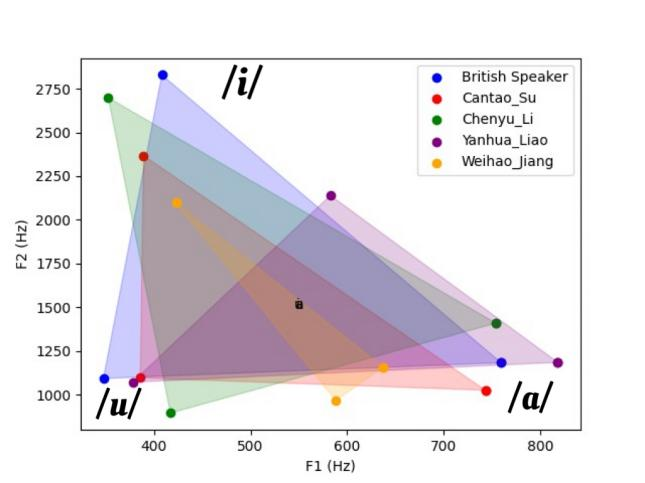
\includegraphics{pic2.jpg}
\caption{VSA Plotting}
\end{figure}
%%%%%%%%%%%%%%%%%%%%%%%%%%%%%%%%%%%%%%%%%%%%%

\bigskip
\textbf{References}:

\noindent Ladefoged, P., \& Johnson, K. (2015). A course in phonetics. Cengage learning.

Liu, H. M., Tsao, F. M., \& Kuhl, P. K. (2005). The effect of reduced vowel working space on speech intelligibility in Mandarin-speaking young adults with cerebral palsy. The Journal of the Acoustical Society of America, 117(6), 3879-3889.

Roy, N., Nissen, S. L., Dromey, C., \& Sapir, S. (2009). Articulatory changes in muscle tension dysphonia: Evidence of vowel space expansion following manual circumlaryngeal therapy. Journal of communication disorders, 42(2), 124-135.


\end{document}
